\documentclass[12pt]{article}
\usepackage{amsmath}
\usepackage{graphicx}
\usepackage{pdfpages}
\usepackage{amssymb}

\title{Exercise Set 7}
\author{Ryan C. Bleile}

\begin{document}
\maketitle

\section{•}
Find the eigenvalues and eigenvectors of the following matrices:

\subsection*{a}

\[
A =
\begin{bmatrix}
7 & 3\\
12 & -2
\end{bmatrix}
\]
\\
Eigenvalues:
\begin{eqnarray*}
0 &=& \det (A - \lambda I )\\
\lambda &=& \frac{5 \pm \sqrt{225}}{2}\\
\lambda_{1} &=& 10\\
\lambda_{2} &=& -5  
\end{eqnarray*}

Eigenvectors:
\[
EV_1 =
\begin{bmatrix}
1\\
1
\end{bmatrix}
EV_2 =
\begin{bmatrix}
1\\
4
\end{bmatrix}
\]

\subsection*{b}

\[
B = 
\begin{bmatrix}
1 & 1\\
1 & 1
\end{bmatrix}
\]

Eigenvalues:
\begin{eqnarray*}
\lambda_1 &=& 0\\
\lambda_2 &=& 2 
\end{eqnarray*}

Eigenvectors:
\[
EV_1 =
\begin{bmatrix}
-1\\
1
\end{bmatrix}
EV_2 =
\begin{bmatrix}
1\\
1
\end{bmatrix}
\]

\subsection*{c}

\[
\begin{bmatrix}
0 & -1\\
1 & 0
\end{bmatrix}
\]

Eigenvalues:
\begin{eqnarray*}
\lambda_1 &=& -i\\
\lambda_2 &=& i
\end{eqnarray*}

Eigenvectors:
\[EV_1 =
\begin{bmatrix}
-i\\
1
\end{bmatrix}
EV_2 =
\begin{bmatrix}
i\\
1
\end{bmatrix}
\]

\section{•}

A non zero 2x2 matrix whose eigenvalues are zero can be found by working backwards from the definition of the eigenvalues.
\begin{eqnarray*}
\lambda^2 &=& 0\\
\lambda^2 + 1 - 1 &=& 0\\
(\lambda +1) (\lambda -1) &=& 0\\
((-1)-\lambda) ((1) -\lambda) + (0)(0) &=& 0
\end{eqnarray*}
\[
\begin{bmatrix}
-1-\lambda & -1\\
1 & 1 - \lambda
\end{bmatrix}
\]

Now using that $0= \det (A-\lambda I)$

\[
\begin{bmatrix}
-1 & -1\\
1 & 1
\end{bmatrix}
-
\lambda
\begin{bmatrix}
1 & 0\\
0 & 1
\end{bmatrix}
\]

So a matrix whose eigenvalues are all zero is:

\[
\begin{bmatrix}
-1 & -1\\
1 & 1
\end{bmatrix}
\]

The eigenvectors of this matrix are in fact only one eigenvector since the eigenvalues are equal. This vector is:

\[
EV = 
\begin{bmatrix}
1\\
-1
\end{bmatrix}
\]

Which when scaled by an arbitrary constant would yield:

\[
EV = \{ C
\begin{bmatrix}
1\\
-1
\end{bmatrix}
\ | \
C \in \mathbb{R \}}
\]

Which is not a basis for $\mathbb{R}^2$ since it is only one vector. It is in fact a basis for one line lying in $\mathbb{R}^2$

\section{•}

Find the matrix whose eigen values are:
\begin{eqnarray*}
\lambda_1 &=& \sqrt{5}\\
\lambda_2 &=& -\sqrt{5}
\end{eqnarray*}
And whose Eigen Vectors are:
\[
EV_1 = 
\begin{bmatrix}
\frac{1 + \sqrt{5}}{2} \\
1
\end{bmatrix}
\ EV_2 =
\begin{bmatrix}
\frac{1 - \sqrt{5}}{2} \\
1
\end{bmatrix}
\]

\[
\begin{bmatrix}
a - \sqrt{5} & b\\
c & d - \sqrt{5}
\end{bmatrix}
\begin{bmatrix}
\frac{1 + \sqrt{5}}{2} \\
1
\end{bmatrix}
=
\begin{bmatrix}
a + \sqrt{5} & b\\
c & d + \sqrt{5}
\end{bmatrix}
\begin{bmatrix}
\frac{1 - \sqrt{5}}{2} \\
1
\end{bmatrix}
\]

\begin{eqnarray*}
(a - \sqrt{5})(\frac{1 + \sqrt{5}}{2}) + b &=& (a + \sqrt{5})(\frac{1 - \sqrt{5}}{2}) + b\\
(c)(\frac{1 + \sqrt{5}}{2}) + (d - \sqrt{5}) &=& (c)(\frac{1 - \sqrt{5}}{2}) + ((d + \sqrt{5})\\
a &=& -\sqrt{5} \\
b &=& 5 + \sqrt{5} \\
c &=& 2\sqrt{5}\\
d &=& -5\\
\end{eqnarray*}

Giving us the Matrix:

\[
A = 
\begin{bmatrix}
-\sqrt{5} & 5 + \sqrt{5} \\
2\sqrt{5} & -5\\
\end{bmatrix}
\]

\section{•}

3 randum matrices:

\subsection*{$1^{st}$}
\[
A1 = 
\begin{bmatrix}
14 & 84\\
25 & 25
\end{bmatrix}
\]
Giving Eigenvalues of:

\begin{eqnarray*}
\lambda_1 &=& \frac{39 - \sqrt{8521}}{2}\\
\lambda_2 &=& \frac{39 + \sqrt{8521}}{2}
\end{eqnarray*}

And a determinant:
$$ \det (A1) = -1750 $$
And Eigenvalues multiplied together gives us:
$$ \frac{39 + \sqrt{8521}}{2} * \frac{39 - \sqrt{8521}}{2} = -1750 $$

This is an interesting result. Lets see if it continues to follow this pattern.

\subsection*{$2^{nd}$}
\[
A2 =
\begin{bmatrix}
81 & 92\\
24 & 34
\end{bmatrix}
\]
Giving Eigenvalues of:

\begin{eqnarray*}
\lambda_1 &=& \frac{115 - \sqrt{11041}}{48}\\
\lambda_2 &=& \frac{115 + \sqrt{11041}}{48}
\end{eqnarray*}

And a Determinant of:
$$ \det (A2) = 546 $$

And Eigenvalues multiplied together gives us:
$$ \frac{115 - \sqrt{11041}}{48} * \frac{115 + \sqrt{11041}}{48} = 546 $$

\subsection*{$3^{rd}$}
\[
A3 =
\begin{bmatrix}
19 & 61\\
25 & 47
\end{bmatrix}
\]
Giving Eigenvalues of:

\begin{eqnarray*}
\lambda_1 &=& \frac{-14-\sqrt{1721}}{25}\\
\lambda_2 &=& \frac{-14+\sqrt{1721}}{25}
\end{eqnarray*}

And a Determinant of:
$$ \det (A3) = -632 $$

And Eigenvalues multiplied together gives us:
$$ \frac{-14-\sqrt{1721}}{25} * \frac{-14+\sqrt{1721}}{25} = -632 $$

\subsection*{Conjecture}

We see from these tree randomly generated matrices that the product of the eigenvalues is equalling the determinant. From this we could say that any randomly generated matrix would have this property. In order to prove this conjecture i will do the following.\\

	We know from solving for the eigenvalues of a matrix that the eigenvalues can always be written as a product of sums. Such that: ($C1 - \lambda$)*($C2 - \lambda$)... = 0 is the product of the sum of a constant term and the eigenvalues of the matrix. This constant term can acctually be solved for for all 2x2 matrices using the quadratic formula. Given that the eigenvalues are a special case of the determinant, when the determinant is equal to zero, we can also say that the determinant of a matrix can be written in this form; such that a $n^{th}$ degree polynomial can be used to represent the determinant of any matrix. Using this we are able to write:
$P(C) = \det (A - CI) $
If we than take the case when the polynomial is at its zero$^{th}$ place i.e. $P(0)$ we can see that the determinant is only be taken on the matrix A.
$$ P(0) = \det (A - 0I) = \det (A) $$

Also if we look back again at our eigenvalues written as a polynomial we see that:
$$ P(0) = (C1 - 0)(C2 - 0)... $$
Which when ($C1 - \lambda$)*($C2 - \lambda$)... = 0, $\lambda_1 = C1$ and $\lambda_2 = C2$ and so on and so forth. So in fact:
$$ P(0) = \lambda_1 * \lambda_2 * ... $$
But we have already found an expression ofr $P(0)$ relating to the determinant. If we combine our two expressions we see that:
$$ \lambda_1 * \lambda_2 * ... = P(0) = \det (A) $$
And in fact the product of our eigenvalues for a matrix A is the determinant of the matrix.

\section{•}

If A has a zero eigenvalue than we can say $A^{-1}$ does not exist. Why?.\\
Starting with the definition of an inverse matrix:
\[
\begin{bmatrix}
a & b\\
c & d
\end{bmatrix}
^{-1}
=
\frac{1}{\det (A)}
\begin{bmatrix}
d & -b\\
-c & a
\end{bmatrix}
\]

Looking at this equation we see that the only time in which the inverse matrix would not exist is if the determinant is equal to zero. This would produce an infinite or undefined result.\\

Using our conjecture above we now know that the determinant of a matrix is found by the product of its eigenvalues. If any or all of the eigenvalues are zero than the product of anything with zero is zero. Therefore the determinant of any matrix with a zero eigenvalue is zero. Since the determinant is zero the matrix has no explicit inverse and therefore does not exist.

\section{•}

Given that two eigenvalues are not equal i.e. ($\lambda_1 \not = \lambda_2$). We can show that the eigenvectors of the matrix will be linearly independent. 

\[
\begin{bmatrix}
a - \lambda_1 & b\\
c & d - \lambda_1
\end{bmatrix}
\begin{bmatrix}
x_1\\
y_1
\end{bmatrix}
= 0
=
\begin{bmatrix}
a - \lambda_2 & b\\
c & d - \lambda_2
\end{bmatrix}
\begin{bmatrix}
x_2\\
y_2
\end{bmatrix}
\] 

This reduces to:
\begin{eqnarray*}
(a-\lambda_1)x_1 + (b)y_1 &=& (a-\lambda_2)x_2 + (b)y_2\\
(c)x_1 + (d-\lambda_1)y_1 &=& (c) x_2 + (d-\lambda_2)y_2 
\end{eqnarray*}

In order to prove that they are linearly independent we will start with the assumption that they are linearly dependant. Meaning that we can write $x_2$, $y_2$ as a scalar multiple of $x_1$, $y_1$; i.e. ($x_2 = C x_1$ and $y_2 = C y_1$).

Using this we can substitute back into the equations above:

\begin{eqnarray*}
(a-\lambda_1)x_1 + (b)y_1 &=& (a-\lambda_2)(C x_1) + (b)(C y_1)\\
(c)x_1 + (d-\lambda_1)y_1 &=& (c) (C x_1) + (d-\lambda_2)(C y_1) 
\end{eqnarray*}

Which we can now simplify and look for an expression to represent the Constant that the second vector would need to be scaled by to become the first. Working through the algebra we see that:

\begin{eqnarray*}
\frac{a-c-\lambda_1}{a-c-\lambda_2} &=& C\\
AND\\
\frac{d-b-\lambda_1}{d-b-\lambda_2} &=& C
\end{eqnarray*}

We can use this expression to show that this cannot be. For if this is true than:

\begin{eqnarray*}
\frac{a-c-\lambda_1}{a-c-\lambda_2} &=& \frac{d-b-\lambda_1}{d-b-\lambda_2}\\
\lambda_1 ((a-c)-(d-b)) &=& \lambda_2 ((a-c)-(d-b))\\
\lambda_1 = \lambda_2
\end{eqnarray*}

This result however is exactly what we defined to not be true. Our first step we have $\lambda_1 \not = \lambda_2$. So it has been shown that two eigenvectors with different eigenvalues cannot be linearly dependant and therefore having two different eigenvalues guarantees that the eigenvectors will be linearly independent. 

\section{•}

If $E_{\lambda}$ is the set of all eigenvectors of a nxn matrix A than it is a vector space. One group of eigenvectors is not a unique solution. In fact the set of all eigenvectors for a matrix is the span of n linearly independent eigenvectors which make up an n dimensional basis.\\

The eigenvectors of a matrix are a set of  vectors which describes each group of dependant equations given by the eigenvalue. These vectors are given by C*one eigenvector solution to the equation, where C can be any constant.\\

We can use one of the first matrices we solved here as an example.

\[
B = 
\begin{bmatrix}
1 & 1\\
1 & 1
\end{bmatrix}
\]

Eigenvalues:
\begin{eqnarray*}
\lambda_1 &=& 0\\
\lambda_2 &=& 2 
\end{eqnarray*}

\begin{eqnarray*}
\lambda_1\\
x_1 + y_1 &=& 0\\
x_1 + y_1 &=& 0\\
\lambda_2\\
-x_1 + y_1 &=& 0\\
x_1 - y_1 &=& 0
\end{eqnarray*}

Eigenvectors:
\[
EV_1 =
\begin{bmatrix}
-1\\
1
\end{bmatrix}
EV_2 =
\begin{bmatrix}
1\\
1
\end{bmatrix}
\]

These eigenvectors are not the only solution to this problem. If we were to scale our eigenvectors by constants say $C_1$ and $C_2$, we would find a new eigenvector set that would be a solution to this problem. If we treat out found eigenvectors like a basis and we find the set of all eigenvectors for this scenario we get:
\[
E_{\lambda} = 
\{ 
C_1
\begin{bmatrix}
-1\\
1
\end{bmatrix}
+
C_2
\begin{bmatrix}
1\\
1
\end{bmatrix}
\ |\ 
C_1 , C_2 \in \mathbb{R}
\}
\]

which is a vector space of $\mathbb{R}^2$, just in our eigenvector basis. We see here that the set of all eigenvectors to a matrix is the span of one set of eigenvectors for that matrix. We have show before that two eigenvectors are linearly independent if their eigenvalues are different. Therefore the set of all eigenvectors for a matrix is a vector space with dimensions equal to the number of distinct eigenvalues from that matrix. Taking the span of a set of eigenvectors fulfils all of the criteria for a vector space. There is a null space, at least trivially when the constants are equal to zero. The eigenvectors are linearly independent and any linear combination of eigenvectors in the space will produce another vector in the same space. Therefore, $E_{\lambda}$ is a vector space.

\section{•}

\begin{figure}[H]
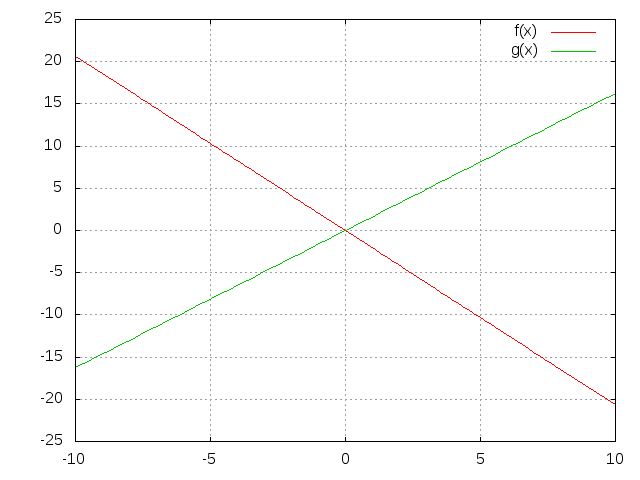
\includegraphics[scale=.35]{eigvec1.png}
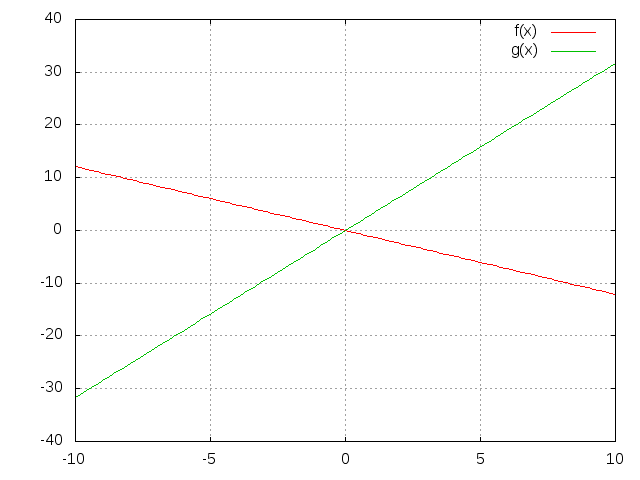
\includegraphics[scale=.35]{eigvec2.png}
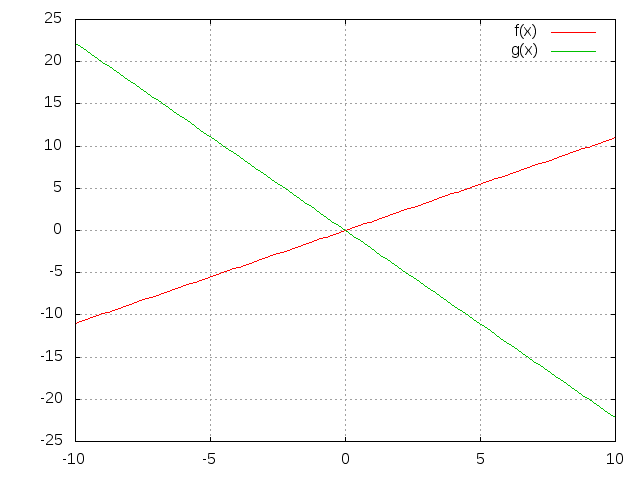
\includegraphics[scale=.35]{eigvec3.png}
\caption{Plots of the Eigen vectors for our three randomly generated matrices in problem 4}
\end{figure}

\clearpage

It appears that a randomly generated all positive matrix will produce perpendicular eigenvectors, where as a matrix which has negative and positive entries will have some angle less than ninety degrees separating them.

This can be checked by preforming the dot product of the eigenvectors in a 2x2 matrix. We will take these three matrices and do the dot product to show that the dot product of two eigenvectors from a matrix produces 0. Which is equivalent to saying that the angle between them is zero.

\[
\begin{bmatrix}
\frac{-11+\sqrt{8521}}{50} & 1
\end{bmatrix}
\begin{bmatrix}
\frac{-11-\sqrt{8521}}{50}\\
1
\end{bmatrix}
\]

\begin{eqnarray*}
\frac{-11-\sqrt{8521}}{50}*\frac{-11+\sqrt{8521}}{50} + 1\\
-(\frac{11+\sqrt{8521}}{50}*\frac{11-\sqrt{8521}}{50})
-1 + 1 &=& 0
\end{eqnarray*}

We can go to show this result for all three of our randomly generated matrices.

If we wish to check the angle between two vectors that are not perpendicular we need to take the arc cosine of the dot product divided by the magnitudes multiplied together. So that:
\begin{eqnarray*}
\theta = \arccos(\frac{\vec{A} \cdot \vec{B}}{AB})
\end{eqnarray*}

Using this we will be able to check a random sample of matrices to see if this conjecture holds any ground.\\

QUESTION:
How is it possible to prove this conjecture. I can not think of a way to show that this is true for all cases. A counter example is enough to show it is false but how does one show that it is true. I have tried working things out generically and did not get anywhere productive.

\end{document}}